\subsection{Vietoris-Rips complex}

We move to our first construction of a filtered simplicial complex, which is built from point cloud data (a subset of points from some metric space).

\begin{definition}[Vietoris-Rips complex]
    Let $(M, d)$ be a metric space, $S \subset M$ be finite, and $\varepsilon > 0$. The \emph{Vietoris-Rips complex} of $S$ at scale $\varepsilon$, denoted $\vr(S; \varepsilon)$, is a simplicial complex defined as
    \[
        \vr(S; \varepsilon) = \left\{
        \sigma \subset S: d(u, v) \leq \varepsilon \;\; \forall u, v \in \sigma
        \right\}.
    \]
\end{definition}

\begin{figure}
    \centering
    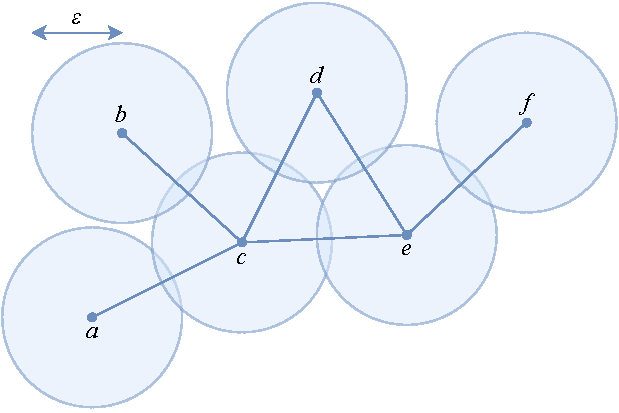
\includegraphics[width=0.7\textwidth]{content/2-background/images/vietoris-rips}
    \caption{Six points with pairwise intersection among balls indicated by a straight edge connecting their centre. The Vietoris-Rips complex fills in all the triangles (one in this example) and higher-dimensional counterparts.}
    \label{fig:vietoris-rips-complex}
\end{figure}

\begin{example}
    Figure \ref{fig:vietoris-rips-complex} shows an example of a Vietoris-Rips complex. In this example, we have
    \begin{align*}
        \restr{\vr(S; \varepsilon)}0 & = \{ \{a\}, \{b\}, \{c\}, \{d\}, \{e\}, \{f\}\},             \\
        \restr{\vr(S; \varepsilon)}1 & = \{ \{a,c\}, \{b,c\}, \{c,d\}, \{c,e\}, \{d,e\}, \{,f\}\}, \\
        \restr{\vr(S; \varepsilon)}2 & = \{ \{c,d,e\} \}.
    \end{align*}
\end{example}

\begin{lemma} \label{lem:vietoris-rips-is-simplicial-complex}
    Any Vietoris-Rips complex is a simplicial complex.
\end{lemma}

\begin{proof}
    Let $(M, d)$ be a metric space, $S \subset M$ be finite, $\varepsilon \geq 0$, and $K = \vr(S; \varepsilon)$. Let $\sigma \in K$ and $\sigma' \subset \sigma$. Trivially, $\varnothing \in K$. Let $u, v \in \sigma'$ be (not necessarily distinct) points. Then $u, v \in \sigma$, so $d(u, v) \leq \varepsilon$. Thus $\sigma' \in K$.
\end{proof}

We now use the Vietoris-Rips complex to form a filtered simplicial complex.

\begin{definition}[Vietoris-Rips filtration] \label{def:filtered-vietoris-rips}
    Let $(M, d)$ be a metric space and $S \subset M$ be finite. Define the \emph{Vietoris-Rips filtration} as $\{\vr(S; \varepsilon)\}_{\varepsilon \in \R_{\geq 0}}$.
\end{definition}

\begin{corollary}[of Lemma \ref{lem:vietoris-rips-is-simplicial-complex}]
    A Vietoris-Rips filtration is a filtered simplicial complex.
\end{corollary}

We now introduce an alternative definition of a filtered Vietoris-Rips complex, by defining a weight function. This will be useful when we consider fast constructions in Section \ref{sec:computing-complexes}.

\begin{definition}[Weight function]
    Let $K$ be a simplicial complex. $w: K \to \R$ is a \emph{weight function} (defined on each simplex of $K$) if $\{w^{-1}(-\infty, \varepsilon]\}_{\varepsilon \in \R}$ is a filtered simplicial complex.
\end{definition}

We call a simplicial complex with a weight function $(K, w)$ a \emph{weight-filtered simplicial complex}.

\begin{definition}[Vietoris-Rips filtration, by weight function] \label{def:filtered-vietoris-rips-weight}
    Let $(M, d)$ be a metric space and $S \subset M$ be finite. We define the filtered Vietoris-Rips complex as $\{w(-\infty, \varepsilon)\}_{\varepsilon \in \R_{\geq 0}}$ where we define the weight function as
    \[ w(\sigma) = \begin{cases}
            0                                  & \text{if $\dim\sigma \leq 0$}  \\
            d(u, v)                            & \text{if $\sigma = \{u, v\}$,} \\
            \max_{\tau \subset \sigma} w(\tau) & \text{otherwise}.
        \end{cases}\]
\end{definition}

\begin{lemma} \label{lem:weight-definition-equivalent}
    Definition \ref{def:filtered-vietoris-rips} and Definition \ref{def:filtered-vietoris-rips-weight} are equivalent.
\end{lemma}

\begin{proof}
    Let $(M, d)$ be a metric space, $S \subset M$ be finite, and $\varepsilon \in \R_{\geq 0}$. We will show that $w^{-1}(-\infty, \varepsilon] = \vr(S;\varepsilon)$. Let $\sigma \subset S$. Trivially, if $\dim\sigma \leq 0$ then $\sigma \in w^{-1}(-\infty, \varepsilon]$ and $\sigma \in \vr(S;\varepsilon)$. Now suppose $\dim\sigma = 1$, so $\sigma = \{u, v\}$ (distinct points). Then $w(\sigma) = d(u,v)$ and so $\sigma \in w^{-1}(-\infty, \varepsilon]$ if and only if $\sigma \in \vr(S;\varepsilon)$. Now suppose $\dim\sigma \geq 2$. Then
    \[ w(\sigma) = \max_{\sigma' \subset \sigma} w(\sigma') = \max_{\{u, v\} \subset \sigma} d(u,v) \]
    and so $w(\sigma) \leq \varepsilon$ if and only if $d(u,v) \leq \varepsilon$ for all $\{u,v\} \subset \sigma$.
\end{proof}
